\documentclass{article}

\usepackage[utf8]{inputenc}
\usepackage[T1]{fontenc}      
\usepackage[francais]{babel}
\usepackage{graphicx}
\usepackage{circuitikz}
\usepackage[squaren, Gray]{SIunits}
\usepackage{sistyle}
\usepackage[autolanguage]{numprint}
\usepackage{pgfplots}
\usepackage{amsmath,amssymb,array}
\usepackage{url} 

% New command pour la modélisation mécanique, tri à effectuer
\newcommand\fv[1]{{\bf #1}} % free vector
\newcommand\fvd[1]{\dot{\bf #1}} % free vector derivated
\newcommand\fvdd[1]{\ddot{\bf #1}} % free vector derivated
\newcommand\fvr[1]{\mathring{\bf #1}} % free vector relatively derivated
\newcommand\fvrr[1]{\overset{\circ\circ}{\bf #1}} % free vector relatively derivated
\newcommand\uv[1]{{\bf\hat{ #1}}} % unit vector
\newcommand\ui{{\bf\hat{I}}} % unit vector I
\newcommand\uj{{\bf\hat{J}}} % unit vector J
\newcommand\uk{{\bf\hat{K}}} % unit vector K
\newcommand\wrt[2]{\ensuremath{\tensor*[_{ #1}]{ #2}{}}} % With Respect To
\newcommand\wtr[3]{\ensuremath{\tensor*[_{ #1}]{ #2}{^{ #3}}}} % With Two Respect
\newcommand\omegaf{{\bm \omega}}
\newcommand\omegafr{\mathring{\bm \omega}}
\newcommand\omegafd{\dot{\bm \omega}}
\newcommand\omegaft{\tilde{\bm \omega}}
\newcommand\omegaftr{\mathring{\tilde{\bm \omega}}}
\newcommand\omegat{\tilde{\omega}}
\newcommand\omegatd{\tilde{\dot{\omega}}}
\newcommand\ine{{\bf I}}
\newcommand\st{{\bf L}}
\newcommand\pst{{\bf M}}
\newcommand\lm{{\bf N}}
\newcommand\am{{\bf H}}
\newcommand\amd{\dot{\am}}
\newcommand\fo{{\bf F}}
\newcommand\po{\mathcal{P}}
\newcommand\xg{\ensuremath{\fv{R}}}
\newcommand\xgd{\ensuremath{\fvd{R}}}
\newcommand\xgdd{\ensuremath{\fvdd{R}}}
\newcommand\dvec[1]{\dot{\vec{ #1}}}
\newcommand\ddvec[1]{\ddot{\vec{ #1}}}
\newcommand\qp{\dot{q}}
\newcommand\dqp{\Delta \dot{q}}

\begin{document}


%La description de l’appareillage de mesure est claire et complète 
Pour pouvoir tester le circuit, nous avons arrangé les appareils comme cela: Nous relions deux générateurs fournissant +15 et 
-15 volts à la plaquette.  Elle même est reliée à la bobine mobile.  La bobine fixe a quand a elle une source de tension qui 
lui fournit un amperage de 1 A pour produire un champs magnétique suffisant.


Concernant les instruments de mesures, on place la pointe de l'oscilloscope sur la sortie de la plaquette et le fréquence
de la musique apparait sur l'écran.  On peut aussi tester le champs électrique passant dans la bobine fixe, on utilise le
teslamètre en mettant le capteur dans l'entrefer, entre la bobine et une barre du 'E'.  On se sert aussi d'un multimetre
pour mesurer la resistance des bobines et du courant qui les traverse.


Nous avons fait de notre mieux pour avoir une aussi bonne précision que possible mais nous savons qu'elle peut être grandement
améliorée, quand nous tenons le teslametre, il est extrèment dur d'obtenir un champs continue, celui-çi varie légerement donc
nous avons pris la valeure la plus centrale mais celle-çi n'est pas très précise.  Pour l'oscilloscope, on doit régler 
la précision de l'appareil si nous voulons être précis.  Même avec cela il est assez difficile de savoir mesurer avec une
très grande précision l'amplitude du signal.

\begin{figure}[ht!]
    \centering
    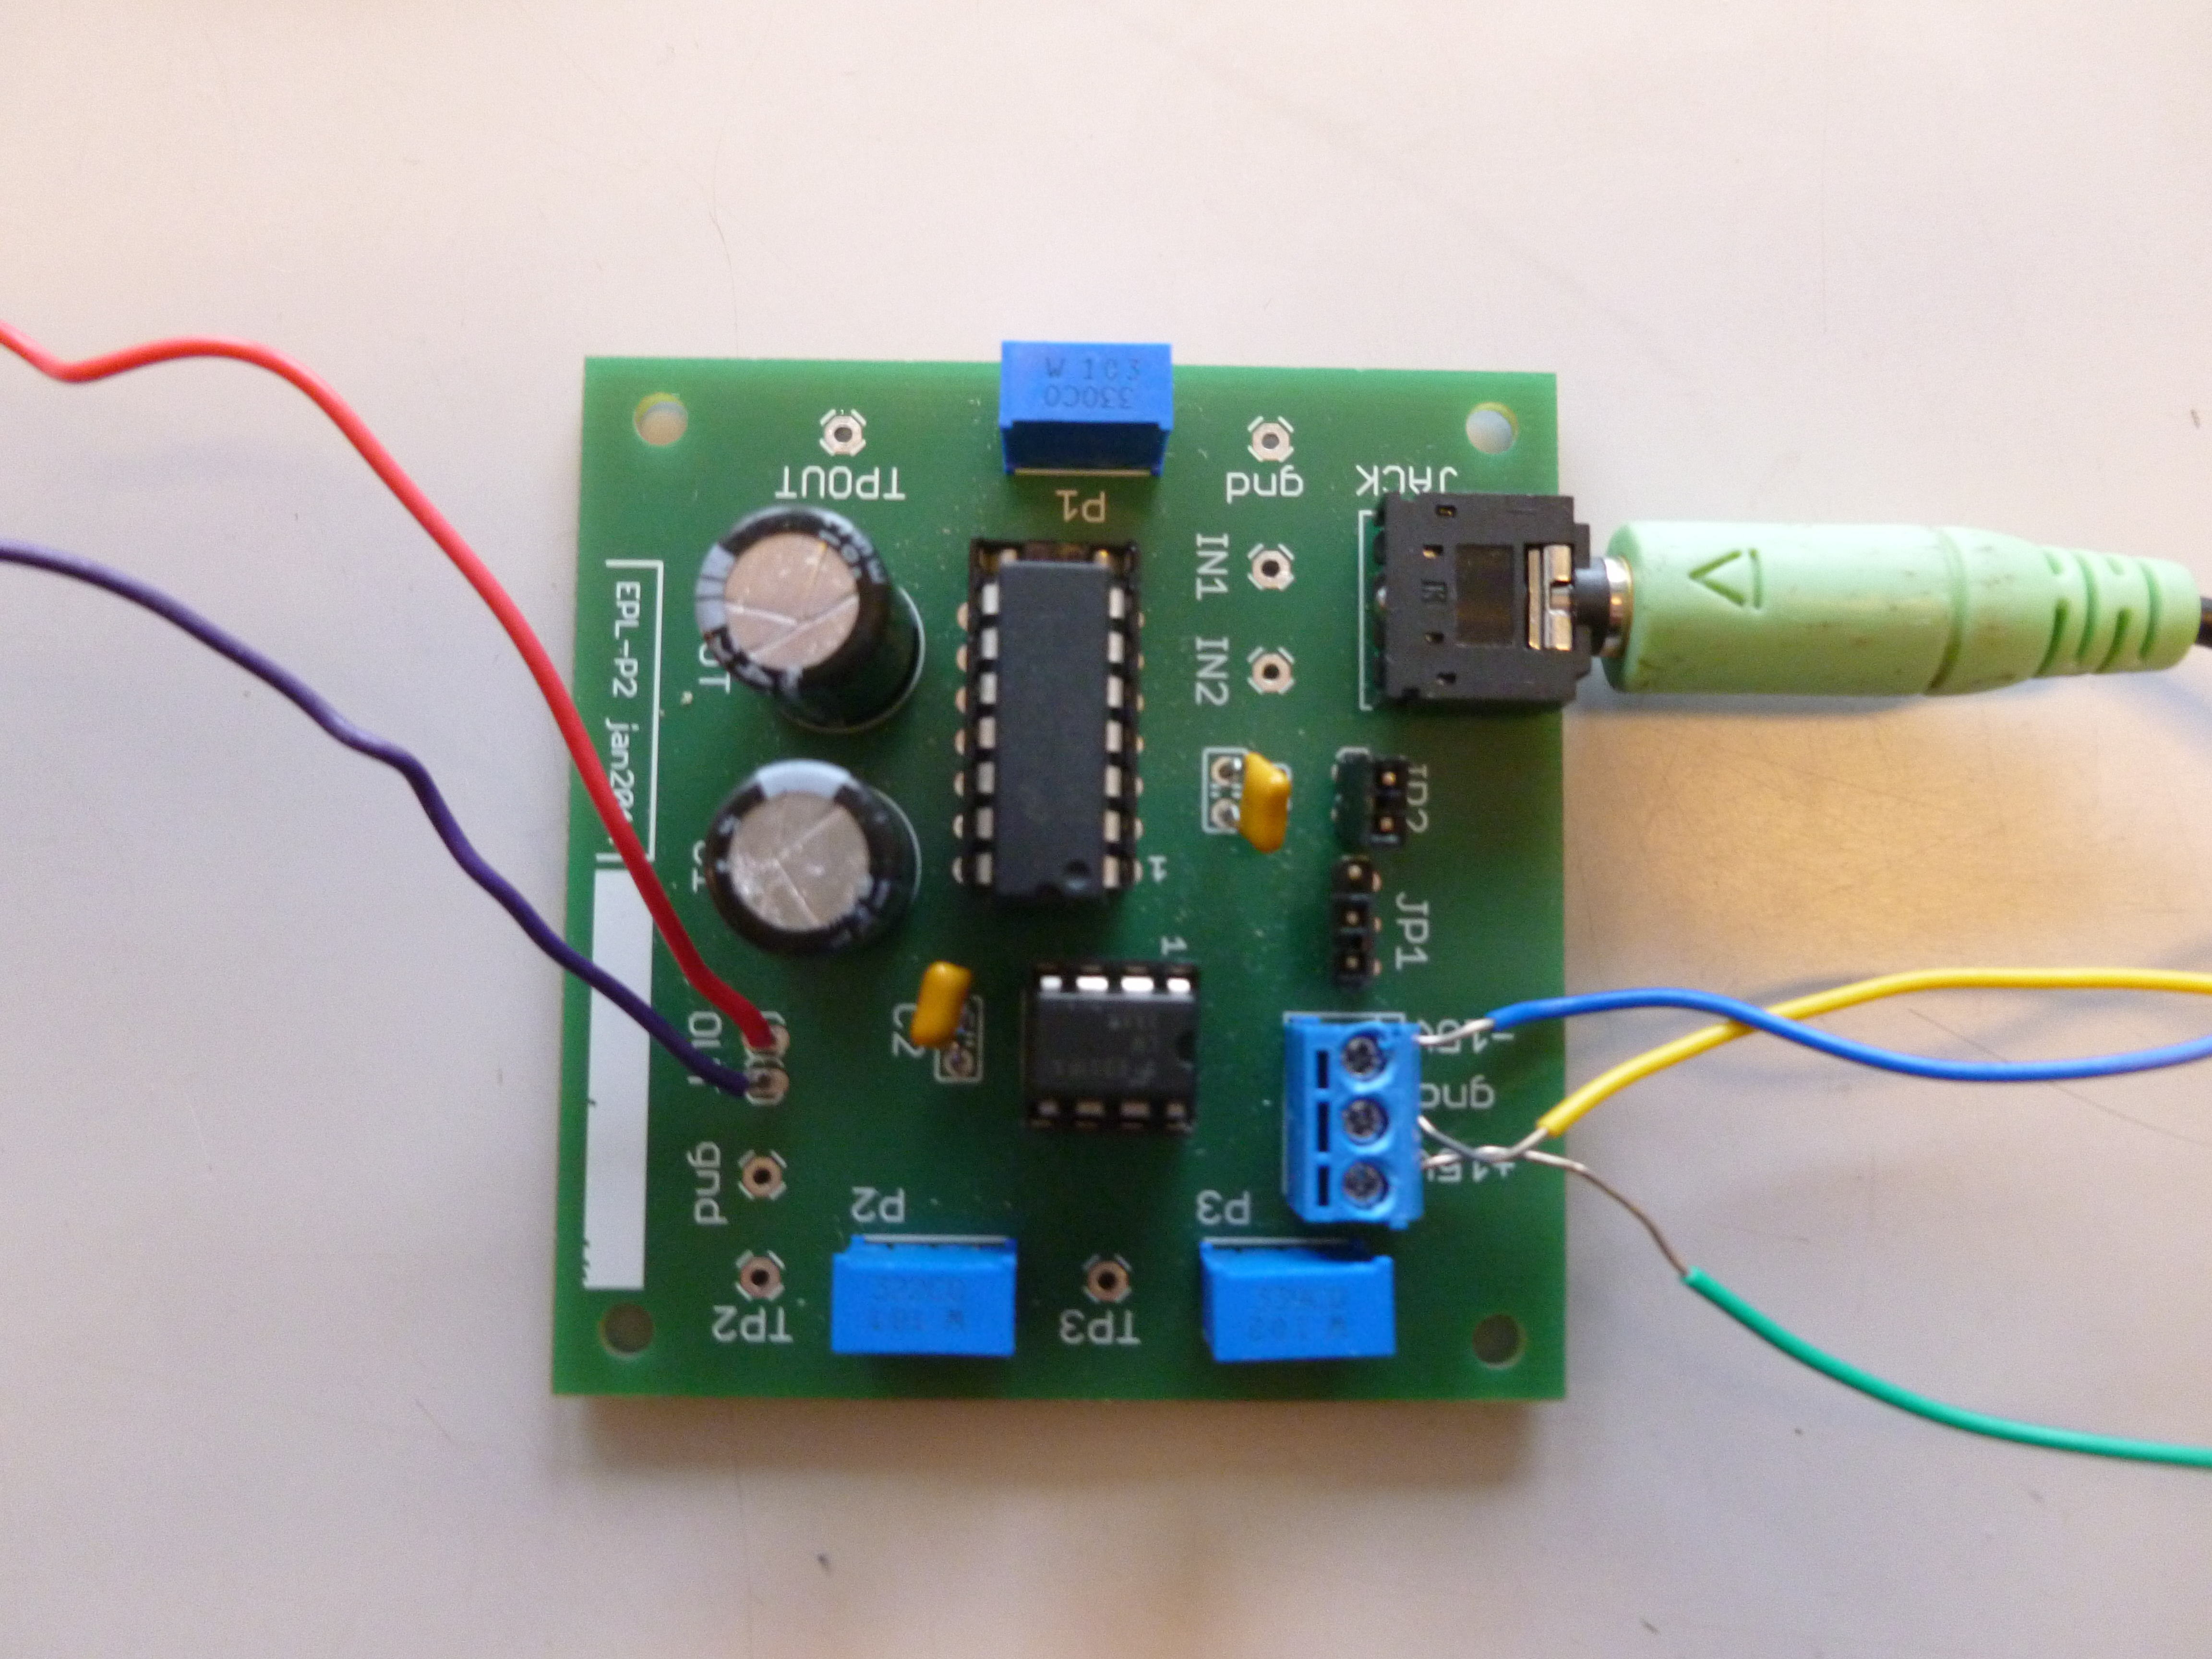
\includegraphics[scale=0.05]{P1010039.jpg}
    \caption{Schéma de la plaquette}
    \label{plaquette}
\end{figure}


%La méthode des mesures est expliquée

Nous avons fait des mesures de voltage en fonction de différentes fréquences pour les filtres RC: ce qui nous a permis
de trouver les fréquences de coupures. Pour mesurer les différentes valeurs reprises ci dessous, nous avons procédé de la
façon suivante: nous avons branché deux générateurs à la plaquette: Une source positive branchée à la borne $+15$ de la plaquette. 
Une source négative branchée à la borne $-15$ de la plaquette.  La terre est quant à elle branchée au dernier point 
disponible de la plaquette: gnd (pour ground).  De plus, la terre est branchée aux sources positives et négatives 
restantes.  Quand nous mesurons la tension aux différents points nous nous servons d'un oscilloscope.  Avec la sonde,
nous touchons le circuit où nous voulons savoir la valeur de la tension.  Sur l'écran, on voit apparaitre le 
signal, en réglant l'appareil sur le bon ordre de grandeur, nous pouvons mesurer assez précisement la tension en 
tel ou tel point.  En annexe, on peut voir des photos des phases de tests. 
  Nous avons fait ces tests avec les filtres
passe haut et passe bas.  Cela correspond au bloc 1 et 2.

\begin{figure}[ht!]
    \centering
    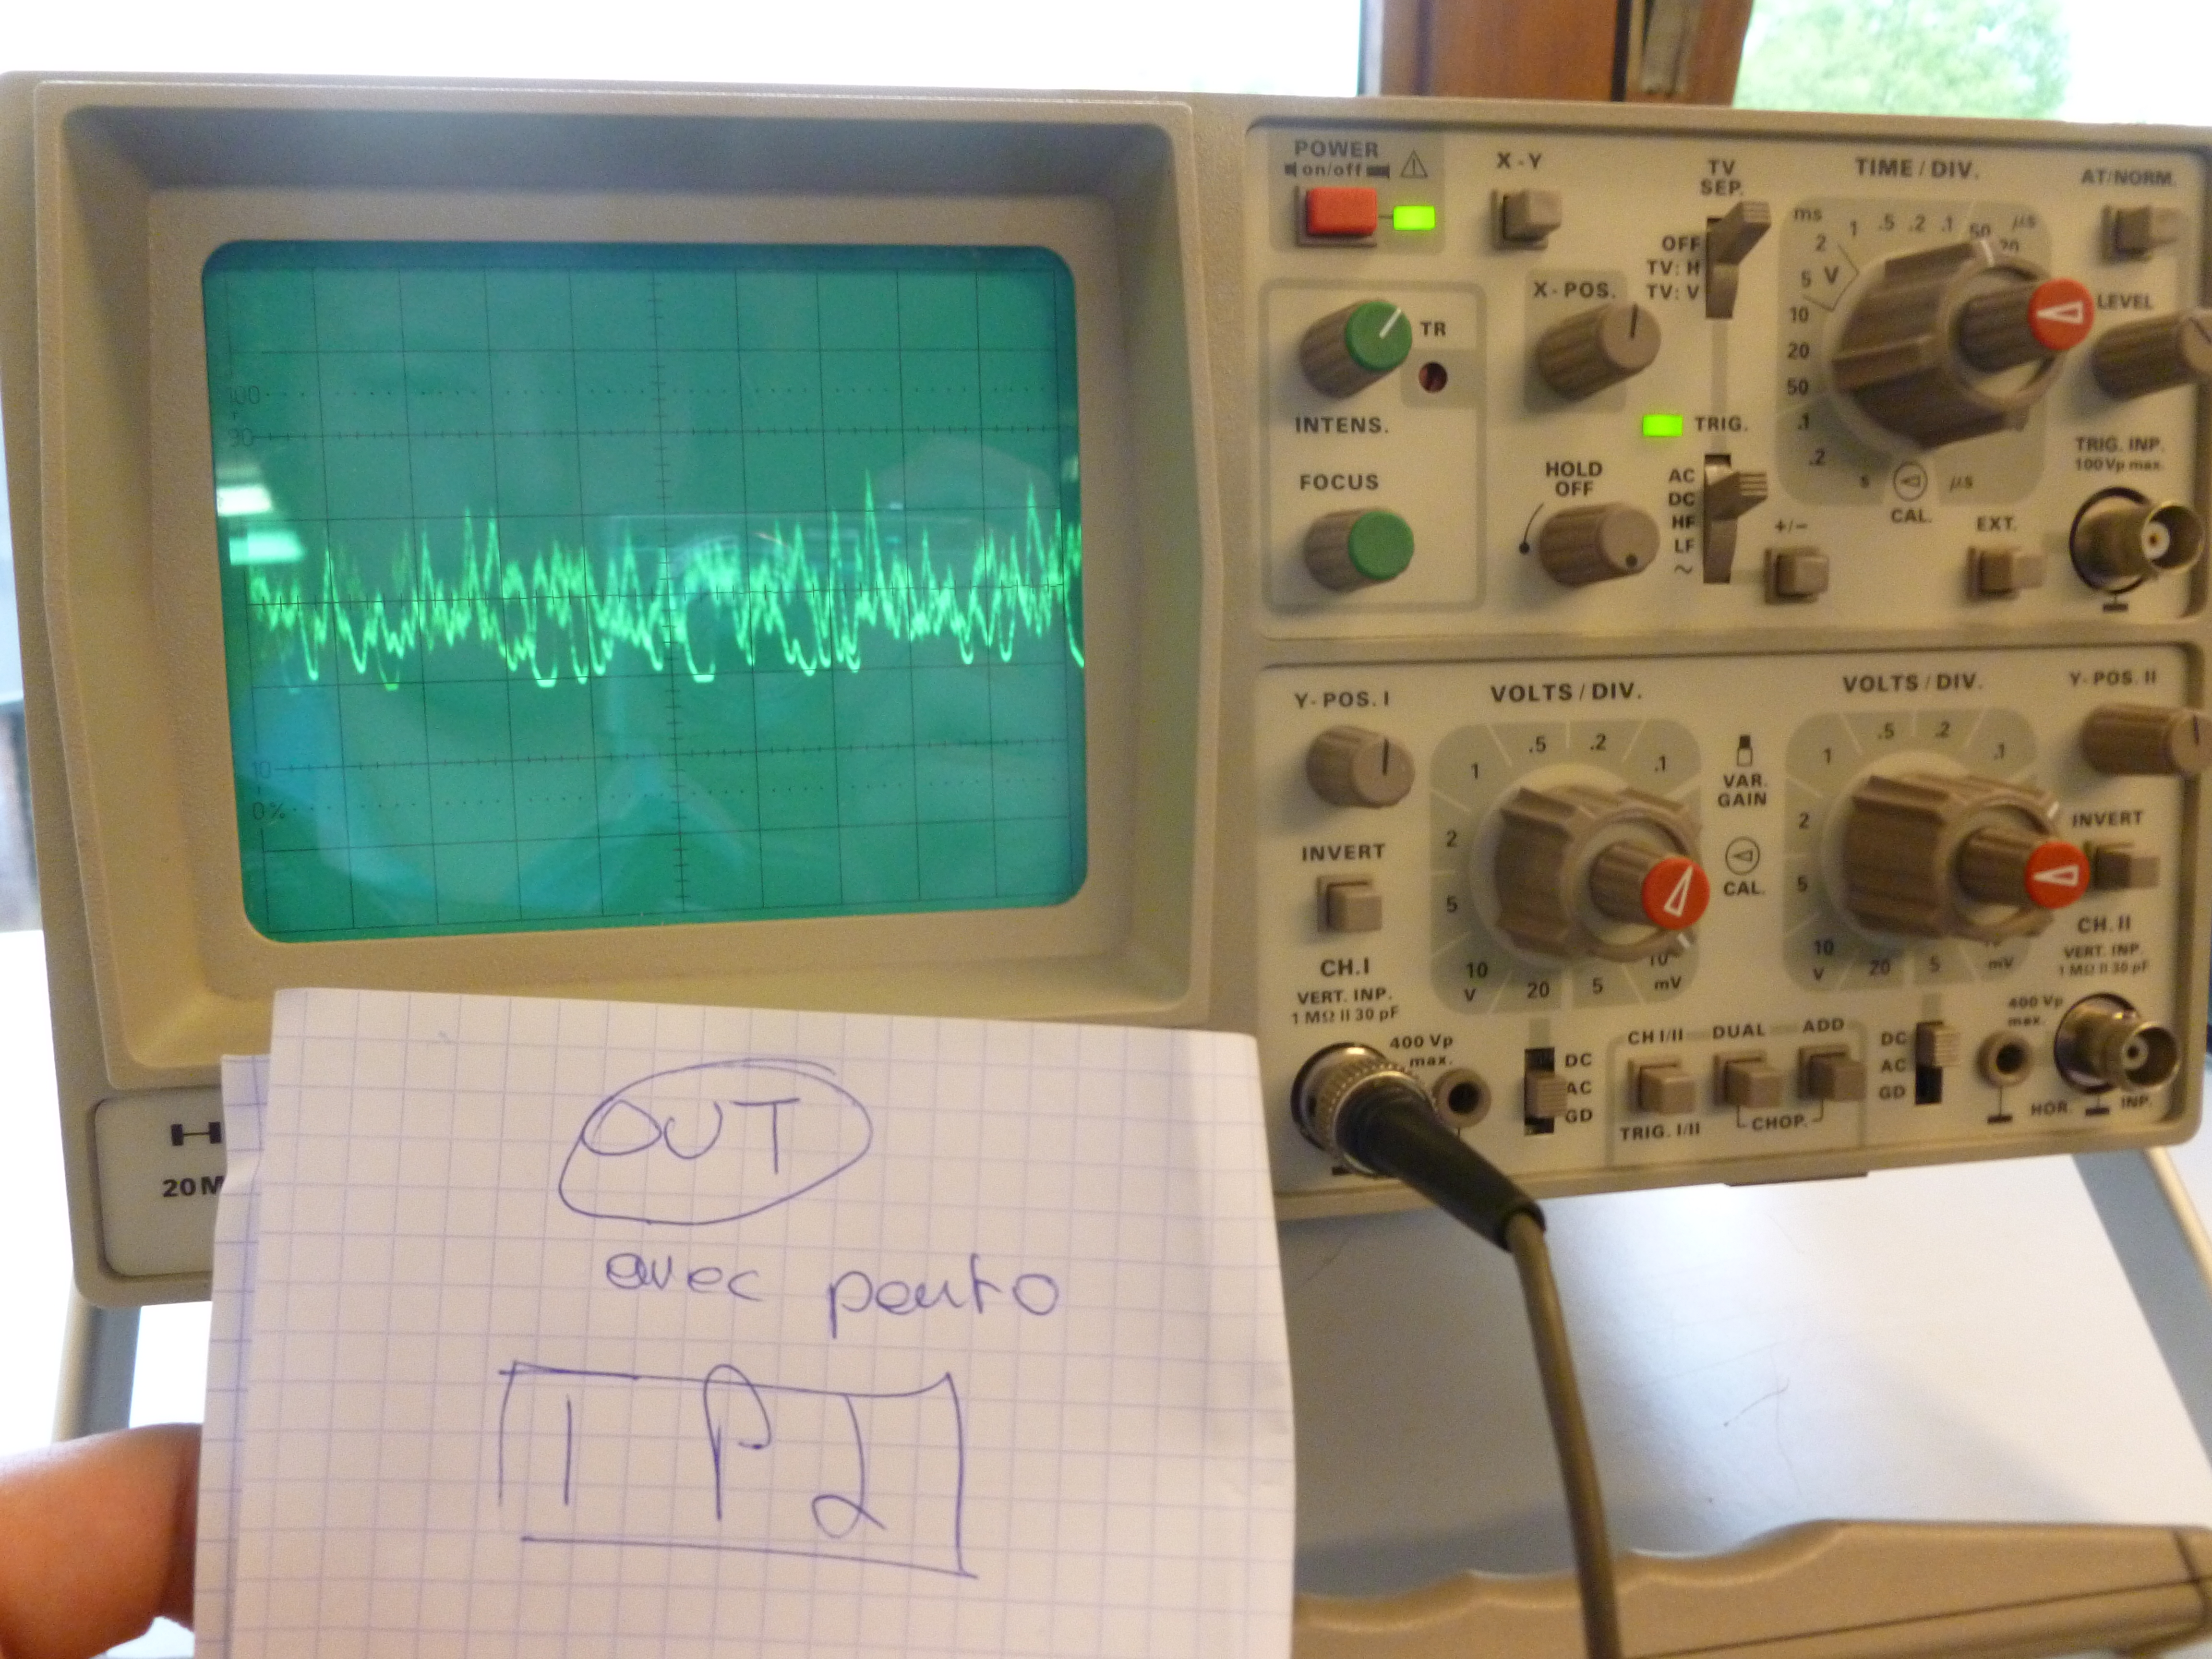
\includegraphics[scale=0.05]{P1010038.jpg}
    \caption{Oscilloscope}
    \label{Oscilloscope pour TP2}
\end{figure}


Pour la bobine fixe, nous voulions savoir quel était le champs produit par les bobines, pour cela nous avons fait passer
du courant dans les bobines en reliant un générateur avec les fils de la bobine et nous avons mis le capteur du teslamètre 
dans l'entrefer.  Après, nous lisions la valeur du champs sur l'écran de l'appareil.
Quand nous mesurions la resistance des bobines, nous isolions la bobine que nous voulions tester, on la branche au multimètre
et on regarde la valeur, nous veillons à chaque fois à bien avoir le bon ordre de grandeur. Cela renvoit au bloc 3.

Enfin, nous avons fait des tests sur la sortie de la plaquette, en testant avec l'oscilloscope.  Nous regardions l'écran de
l'appareil pour voir si une fréquence possible sortait de la plaquette.  Cela correspond au bloc 4.

\emph{Précautions}
\begin{enumerate}
\item Lors de chaque test, il est nécessaire de laisser les objets immobiles pour éviter des erreurs dû à leur mobilité.
\item Eviter que les fils ne touchent la plaque verte, qui est la masse.


%Des tests paramétriques sont effectués

Nous avons décidé de faire nos essais avec une tension de plus et moins 15 V car l'ampli-op nécéssite une tension
de maximum plus et moins 16.5 V, nous prenons un peu moins pour avoir une marge de sécurité.
Il est clair que si nous changeons cette valeure et que nous mettons plus de tension, le son sera plus amplifié vu que 
la plaquette aura une plus grande source de tension.  


En faisant augmenter les aigus, nous voyons que le signal est plus condensé et vice versa.

Quand nous mettons plus de courant dans la bobine fixe, un plus grand champs magnétique est créé, mais trop l'augmenter
ferait fondre le fil.

\begin{figure}[ht!]
    \centering
    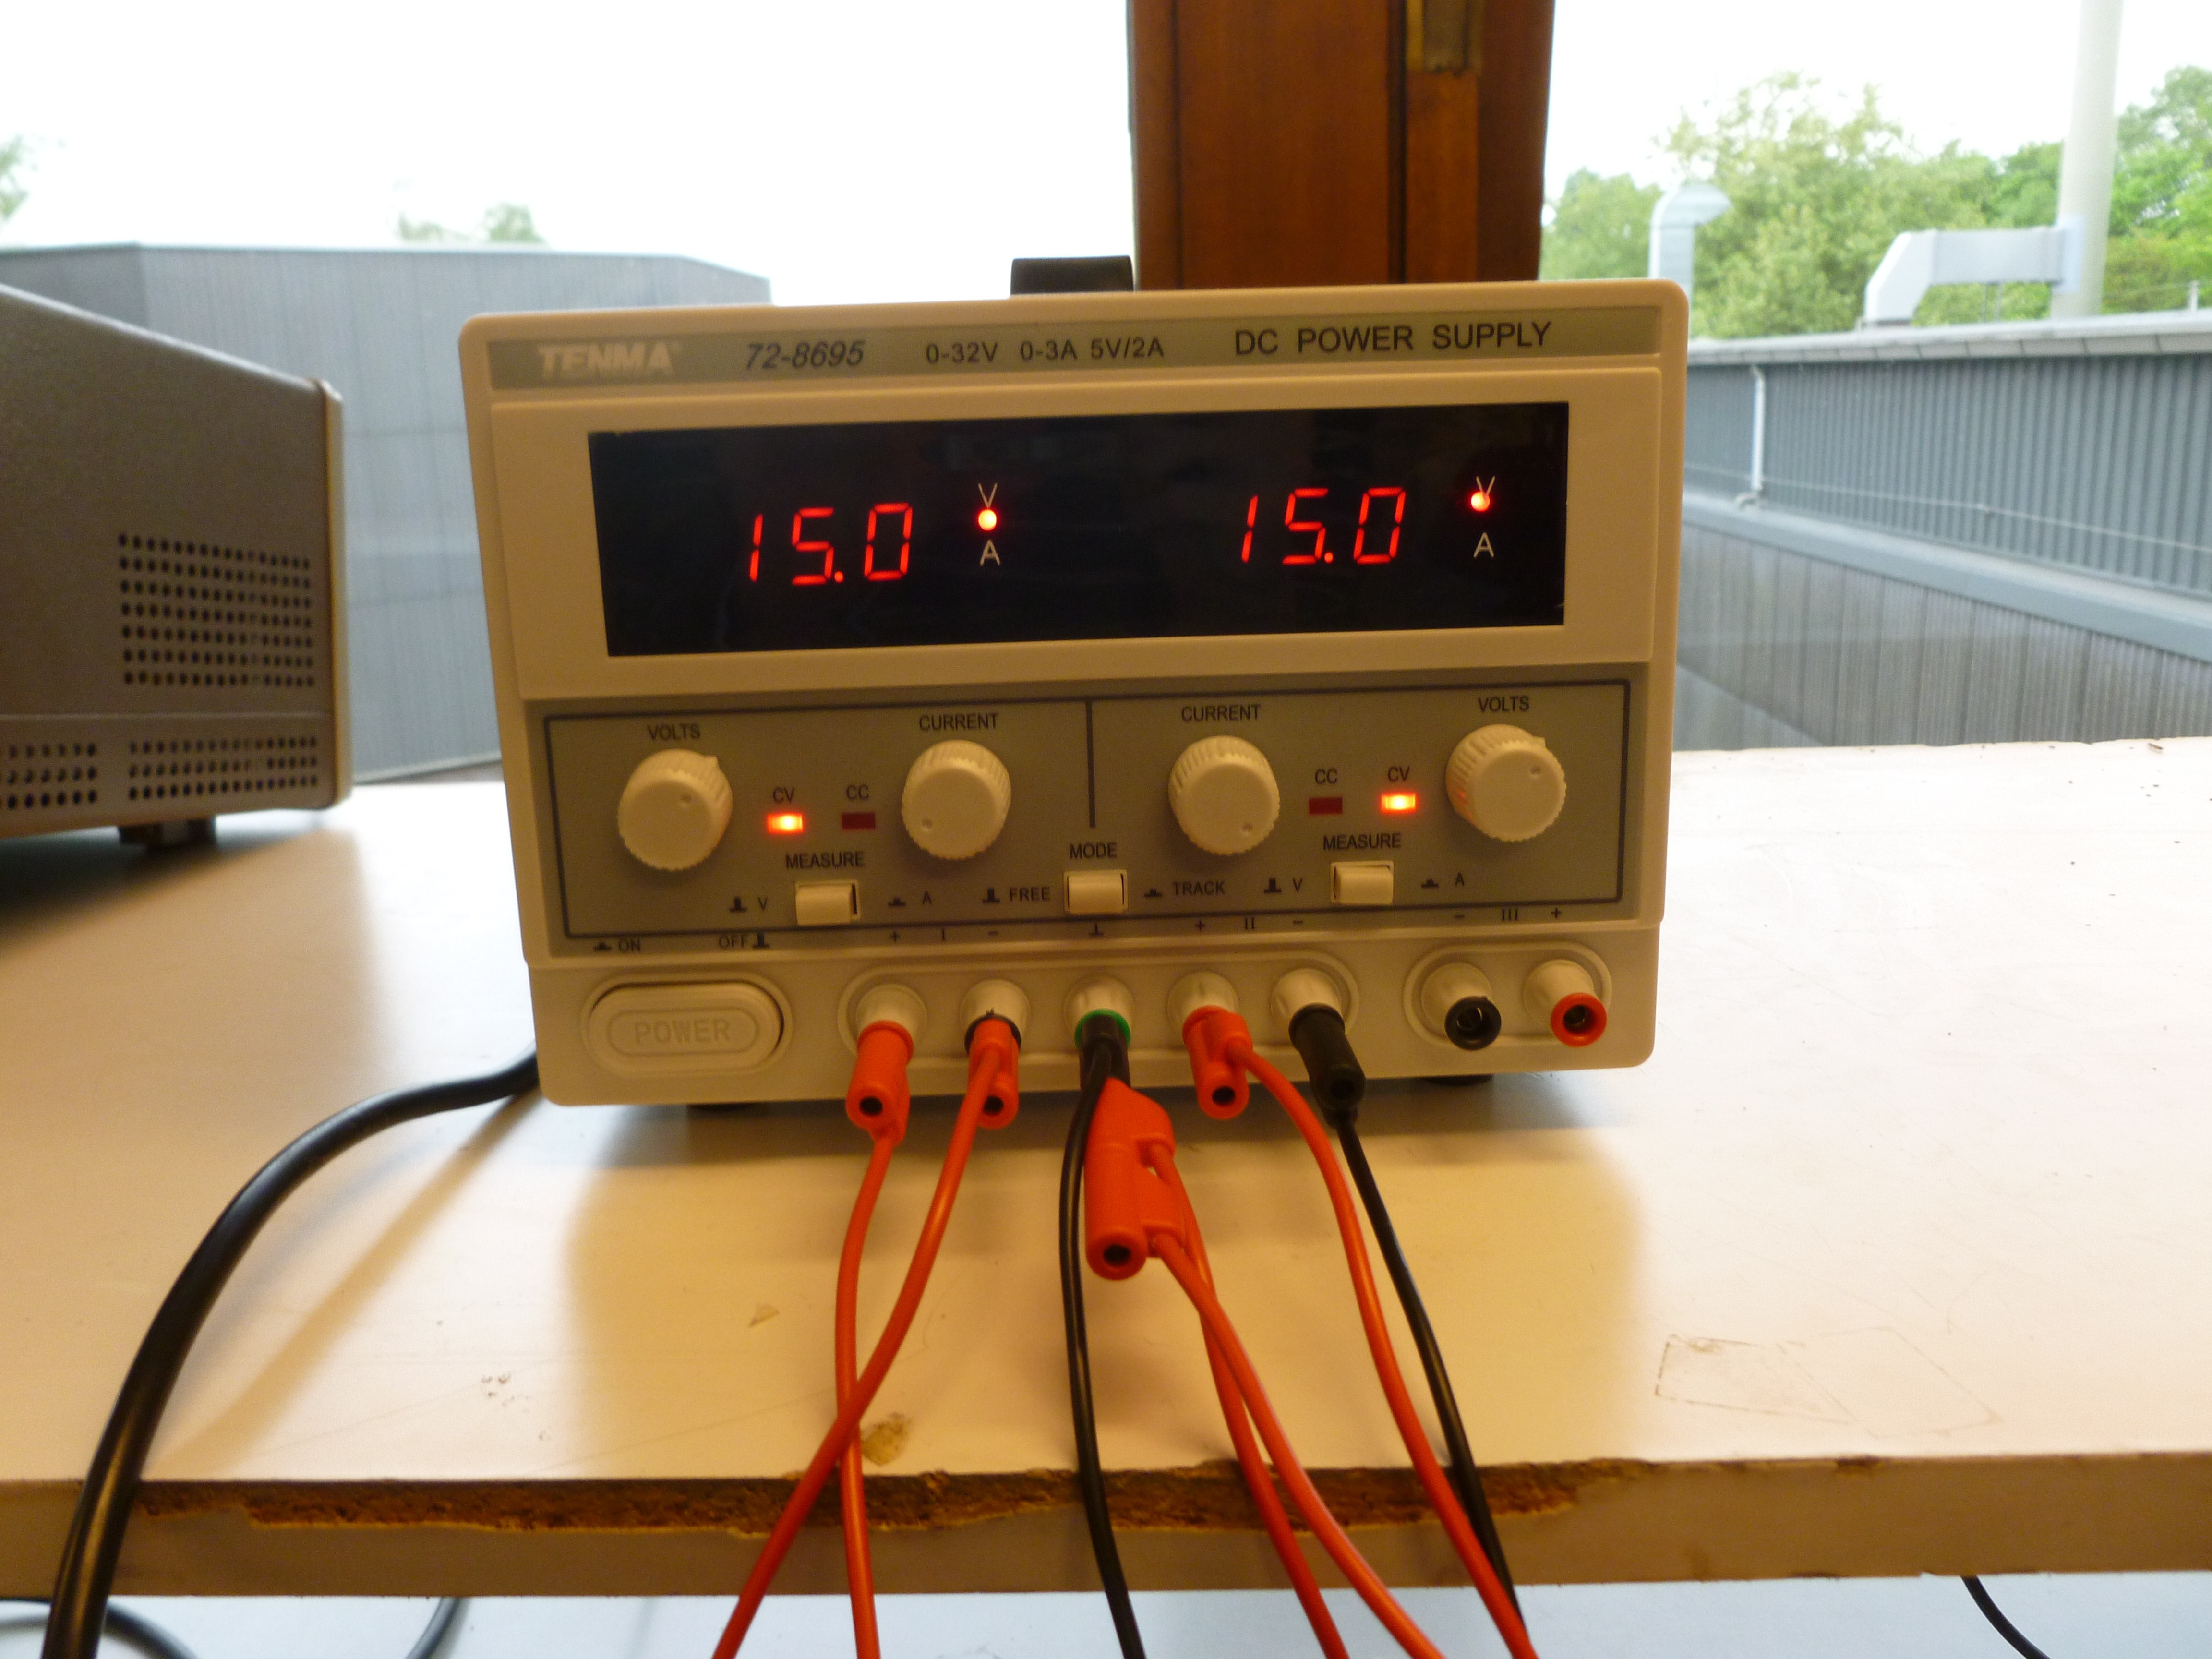
\includegraphics[scale=0.05]{P1010031.jpg}
    \caption{Générateurs}
    \label{Branchements des générateurs}
\end{figure}

%Mesures
Pour le filtre passe-bas:
\begin{center}
\begin{tabular}{|c|c|c|}
\hline
$V_c[V]$ & $f[Hz]$ & $\log{f}$ \\
\hline
1.7 & 16000 & 4.204 \\
\hline
1.55 & 18000 & 4.255 \\
\hline
1.45 & 20000 & 4.301 \\
\hline
\end{tabular}
\end{center}

Pour le filtre passe-haut

\begin{center}
	\begin{tabular}{|c|c|c|}
		\hline
		$V_c[V]$ & $f[Hz]$ & $\log{f}$ \\
		\hline
		127 & 0.4 & 2.1\\
		\hline
		191 & 0.5 & 2.3\\
		\hline
		356 & 0.6 & 2.6 \\
		\hline
	\end{tabular}
\end{center}

\begin{center}
	\begin{tabular}{|c|c|c|}
		\hline
		$Resistance bobine fixe[\ohms]$ & $Champ magn.[T]$ & $Amperage[A]$ \\
		\hline
		2.38 & 0.08 & 0.1667\\
		\hline
	\end{tabular}
\end{center}

\begin{document}

\begin{center}
\begin{tabular}{|c|c|c|c|c|}
\hline
$Prise Jack [mV]$ & $IN_1 [mV]$ & $OUT_{avec  pentotiomètre} [V]$ & $OUT_{sans pentotiomètre} [V]$ & $TP_2 [mV]$ \\
		\hline
		 37.5 & 100.0 & 0.22 & 3.0 & 11.0 \\
		\hline
	\end{tabular}
\end{center}





% Just here to fix rapport_prejury.tex
\end{document}
